\documentclass[11pt]{beamer}

\usetheme{Warsaw}
\setbeamertemplate{page number in head/foot}[totalframenumber]

\usepackage[utf8]{inputenc}
\usepackage[T1]{fontenc}
\usepackage[french]{babel}
\usepackage{amsmath}
\usepackage{amsfonts}
\usepackage{amssymb}
\usepackage{graphicx}
\usepackage{geometry}
\usepackage{listings, lstautogobble}
\usepackage[strings]{underscore}

\lstset{
	language=Python,
	frame=single,
	numbers=left,
	tabsize=4,
    autogobble=true,
	showstringspaces=false
}

\title{Implémentation de\\l'algorithme de Dijkstra et sa variante A*\\en Python 3 et Tkinter}
\author{Boisnier Thomas}

\begin{document}

\begin{frame}[noframenumbering]
	\thispagestyle{empty}
	\titlepage
\end{frame}

\begin{frame}
	\tableofcontents
\end{frame}

\section{Algorithmes}
	\subsection{Composants}
		\begin{frame}
			L'algorithme de Dijkstra et sa variante A* nécessite plusieurs élements :
			\begin{itemize}
		        \item[•] un point de départ
		        \item[•] un point d'arrivé
		        \item[•] un calcul de distance : coût G
		        \item[•] une heuristique : coût H (uniquement pour A*)
		        \item[•] une liste dite fermée, qui contiendra les points visités
		        \item[•] une liste dite ouverte (file à priorité), qui contiendra les points accessibles \\ (tri croissant du coût total : coût F = coût G + coût H)
			\end{itemize}
		\end{frame}
	
	\subsection{Distance}
		\begin{frame}
			Calcul de la distance (coût G) entre 2 points :
			\begin{itemize}
				\item[•] 1 dans toutes les directions
				\item[•] 1 en horizontale et verticale, sqrt(2) en diagonale
			\end{itemize}
		\end{frame}
		
	\subsection{Heuristique}
		\begin{frame}[fragile]
			Si A* utilise une heuristique (coût H) qui ne surestime jamais la distance du but, A* peut être avéré admissible.
			\vspace{4mm}
			\begin{small}
				\begin{lstlisting}
					dx = abs(node.m_x - target.m_x)
        			dy = abs(node.m_y - target.m_y)
				\end{lstlisting}
			\end{small}	
			\vspace{4mm}
			\begin{center}	
				\begin{tabular}{l|r}
					\hline
					Manhattan & dx + dy\\
					\hline
					Chebyshev & (dx + dy) - min(dx, dy)\\
					\hline
					Octile & (dx + dy) + (sqrt(2) - 2) * min(dx, dy)\\
					\hline
					Euclidean & sqrt(dx * dx + dy * dy)\\
					\hline
				\end{tabular}
			\end{center}
		\end{frame}
		
	\subsection{Déroulement}
		\begin{frame}
			\begin{center}
				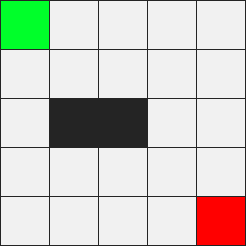
\includegraphics[scale=0.5]{images/Algo_1.png}
				\hspace{1cm}
				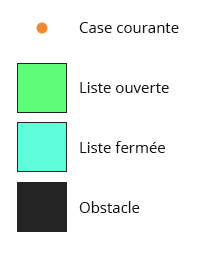
\includegraphics[scale=0.5]{images/Legend.png}
			\end{center}
		\end{frame}
		\begin{frame}
			\begin{center}
				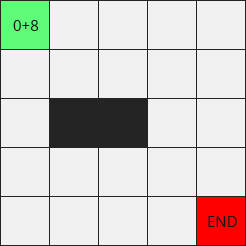
\includegraphics[scale=0.5]{images/Algo_2.png}
				\hspace{1cm}
				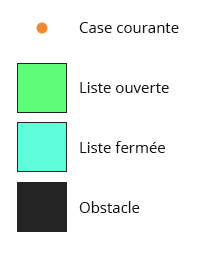
\includegraphics[scale=0.5]{images/Legend.png}
			\end{center}
		\end{frame}
		\begin{frame}
			\begin{center}
				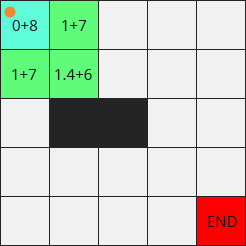
\includegraphics[scale=0.5]{images/Algo_3.png}
				\hspace{1cm}
				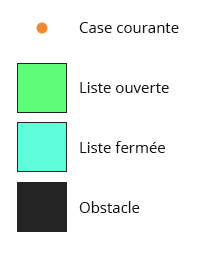
\includegraphics[scale=0.5]{images/Legend.png}
			\end{center}
		\end{frame}
		\begin{frame}
			\begin{center}
				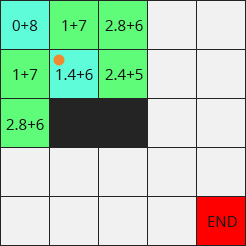
\includegraphics[scale=0.5]{images/Algo_4.png}
				\hspace{1cm}
				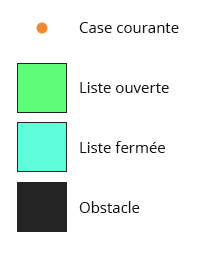
\includegraphics[scale=0.5]{images/Legend.png}
			\end{center}
		\end{frame}
		\begin{frame}
			\begin{center}
				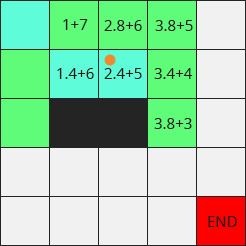
\includegraphics[scale=0.5]{images/Algo_5.png}
				\hspace{1cm}
				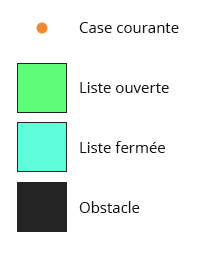
\includegraphics[scale=0.5]{images/Legend.png}
			\end{center}
		\end{frame}
		\begin{frame}
			\begin{center}
				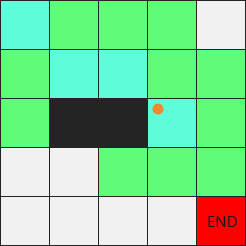
\includegraphics[scale=0.5]{images/Algo_6.png}
				\hspace{1cm}
				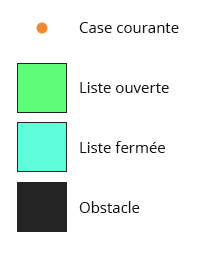
\includegraphics[scale=0.5]{images/Legend.png}
			\end{center}
		\end{frame}
		\begin{frame}
			\begin{center}
				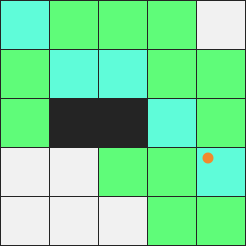
\includegraphics[scale=0.5]{images/Algo_7.png}
				\hspace{1cm}
				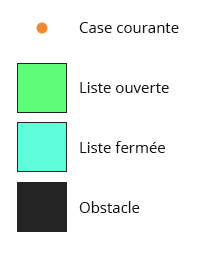
\includegraphics[scale=0.5]{images/Legend.png}
			\end{center}
		\end{frame}
		\begin{frame}
			\begin{center}
				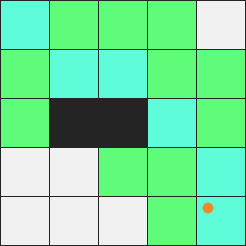
\includegraphics[scale=0.5]{images/Algo_8.png}
				\hspace{1cm}
				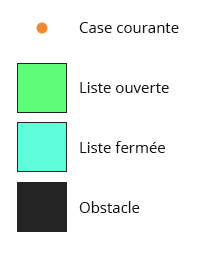
\includegraphics[scale=0.5]{images/Legend.png}
			\end{center}
		\end{frame}		
		
\section{Historique}
	\subsection{Principe}
		\begin{frame}[fragile]
			Historique des actions importantes.
			\begin{itemize}
				\item[•] Historique : Liste contenant les actions
				\item[•] Action : Structure contenant les informations que l'on souhaite (temps, type, ...)
			\end{itemize}
			\vspace{4mm}
			Appel d'une fonction au cours du déroulement de l'algorithme qui ajoute une action à l'historique.	 
			\begin{lstlisting}
				history.add(action_type, cell, time)
			\end{lstlisting}
		\end{frame}
		
\section{Tkinter}
	\subsection{Organisation}
		\begin{frame}
			\begin{center}
				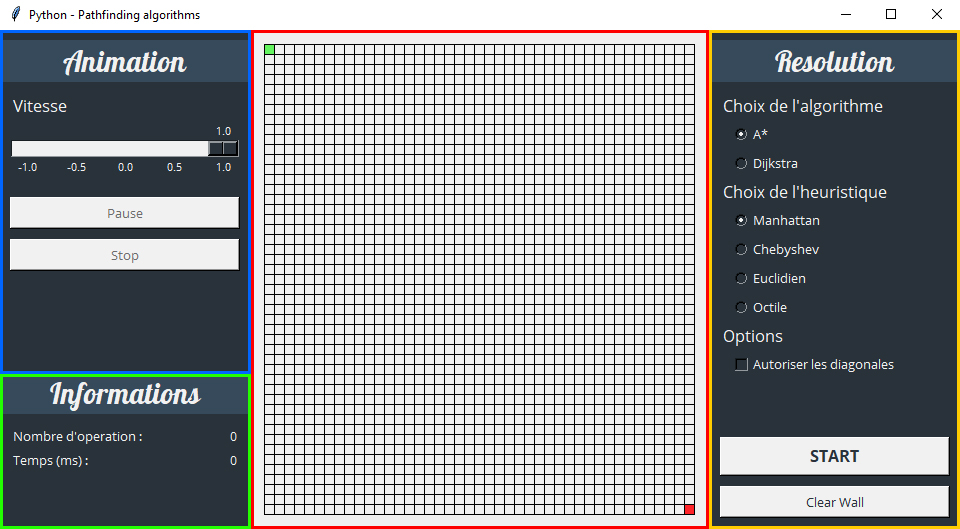
\includegraphics[scale=0.3]{images/UI.jpg}
			\end{center}
			Composants : Menu d'animation (bleu), Cadre des informations (vert), Grille (rouge), Menu de choix de résolution (jaune)		
		\end{frame}

\section{Progression}
	\begin{frame}
		Organisation de l'avancement du projet :
		\begin{itemize}
			\item Documentation
			\item Création de la grille et avec le menu de résolution
			\item Gestion des événements (déplacement des cases de départ/arrivée, création/suppression des obstacles)
			\item Implémentation de l'algorithme A* (rendu en temps réel)
			\item Implémentation d'un historique
			\item Gestion de l'animation
			\item Ajout d'un fichier de configuration
		\end{itemize}
	\end{frame}

\end{document}